% =====================================================================
%  mamadou_maxstables.tex  —  fichier AUTONOME (compiler avec XeLaTeX)
%  Partie : Processus max-stables
% =====================================================================
\documentclass[11pt,a4paper]{article}

% --- préambule (XeLaTeX + français) ---
\usepackage{fontspec}
\setmainfont{Latin Modern Roman}
\usepackage{polyglossia}
\setmainlanguage{french}
\usepackage{amsmath,amssymb,amsthm}
\usepackage{geometry}
\geometry{margin=2.5cm}
\usepackage{graphicx}
\usepackage[hidelinks]{hyperref}

% --- où chercher les figures (plusieurs chemins possibles) ---
\graphicspath{{figures/mamadou_figures/}{mamadou_figures/}{../figures/mamadou_figures/}{./}}

% --- environnements de théorème ---
\newtheorem{theoreme}{Théorème}
\newtheorem{definition}[theoreme]{Définition}

% --- macros ---
\newcommand{\R}{\mathbb{R}}
\newcommand{\E}{\mathbb{E}}
\newcommand{\PP}{\mathbb{P}}
\newcommand{\LN}{L_N}

\title{Processus max-stables}
\author{Mamadou Lamine Kebe \\ \small Projet TVE — Mesures de risque spatiales}
\date{\today}

\begin{document}
\maketitle

\section{Processus max-stables}

Cette partie assure le passage de la théorie des valeurs extrêmes univariée à sa
version spatiale. L'idée directrice tient en une phrase : \emph{un processus
max-stable est à un champ spatial ce que la loi GEV est à une seule variable}.
Là où le cours donne la loi du maximum en un point, on décrit ici le
comportement conjoint des maxima en tout point d'une région.

\subsection{Définition et convergence}

On note $\bigvee$ le supremum, et $\overset{d}{=}$, $\overset{d}{\to}$ l'égalité
et la convergence en loi.

\begin{definition}[Processus max-stable]
Un processus $\{G(\mathbf x)\}_{\mathbf x\in\R^d}$ est \emph{max-stable} s'il
existe des suites de fonctions continues $a_T(\mathbf x)>0$ et $b_T(\mathbf x)$
telles que, pour des répliques indépendantes $G_1,\dots,G_T$ de $G$,
\[
\left\{\frac{\bigvee_{t=1}^T G_t(\mathbf x)-b_T(\mathbf x)}{a_T(\mathbf x)}\right\}_{\mathbf x\in\R^d}
\;\overset{d}{=}\; \{G(\mathbf x)\}_{\mathbf x\in\R^d}.
\]
\end{definition}

Autrement dit, prendre le maximum ponctuel de plusieurs copies indépendantes,
puis renormaliser, redonne le même processus en loi : c'est la max-stabilité du
cours, mais portée par un \emph{champ} entier et non plus par un nombre.

Le résultat fondamental justifie l'emploi de ces processus : si le maximum
ponctuel renormalisé de $n$ répliques indépendantes d'un processus quelconque
converge vers un processus non dégénéré, alors ce processus limite est
\emph{nécessairement} max-stable (de Haan, 1984). C'est l'analogue spatial exact
du théorème de Fisher--Tippett--Gnedenko : la GEV est la seule limite du maximum
d'une variable, le processus max-stable est la seule limite du maximum d'un
champ. En pratique, le nombre $n$ dépend de la période considérée (classiquement
$T_L=1$ an, $n=365$). On appelle \emph{simple} un processus max-stable dont les
marges sont de Fréchet standard, $\PP(Z(\mathbf x)\le z)=\exp(-1/z)$ ; c'est le
cadre de toute la suite.

\subsection{Représentation spectrale}

Comment fabriquer concrètement de tels processus ? La \emph{représentation
spectrale} en donne la recette universelle.

\begin{theoreme}[Représentation spectrale, de Haan 1984]\label{th:spectral}
Tout processus max-stable simple (séparable en probabilité) s'écrit
\begin{equation}\label{eq:spectral}
\{Z(\mathbf x)\}_{\mathbf x\in\R^d}
\;\overset{d}{=}\;
\left\{\bigvee_{i=1}^{\infty} U_i\,V_{\mathbf x}(S_i)\right\}_{\mathbf x\in\R^d},
\end{equation}
où les $(U_i,S_i)_i$ sont les points d'un processus de Poisson d'intensité
$u^{-2}\,\mathrm du\times\mu(\mathrm ds)$, et les $V_{\mathbf x}$ vérifient
$\int V_{\mathbf x}\,\mathrm d\mu=1$ pour tout $\mathbf x$.
\end{theoreme}

L'intuition est physique et se lit sur la figure~\ref{fig:spectral}. Chaque terme
$U_i\,V_{\mathbf x}(S_i)$ est une \emph{« tempête » élémentaire} : une bosse
d'amplitude aléatoire $U_i$, centrée en une position aléatoire $S_i$, dont la
forme décroît avec la distance. Le champ $Z$ est le \emph{maximum} de toutes ces
tempêtes : en chaque point, on ne retient que la plus violente. C'est le
maximum, et non la somme, qui fait la nature \emph{max}-stable du processus. La
condition $\int V_{\mathbf x}\,\mathrm d\mu=1$ garantit que chaque marge est de
Fréchet standard.

\begin{figure}[htbp]
  \centering
  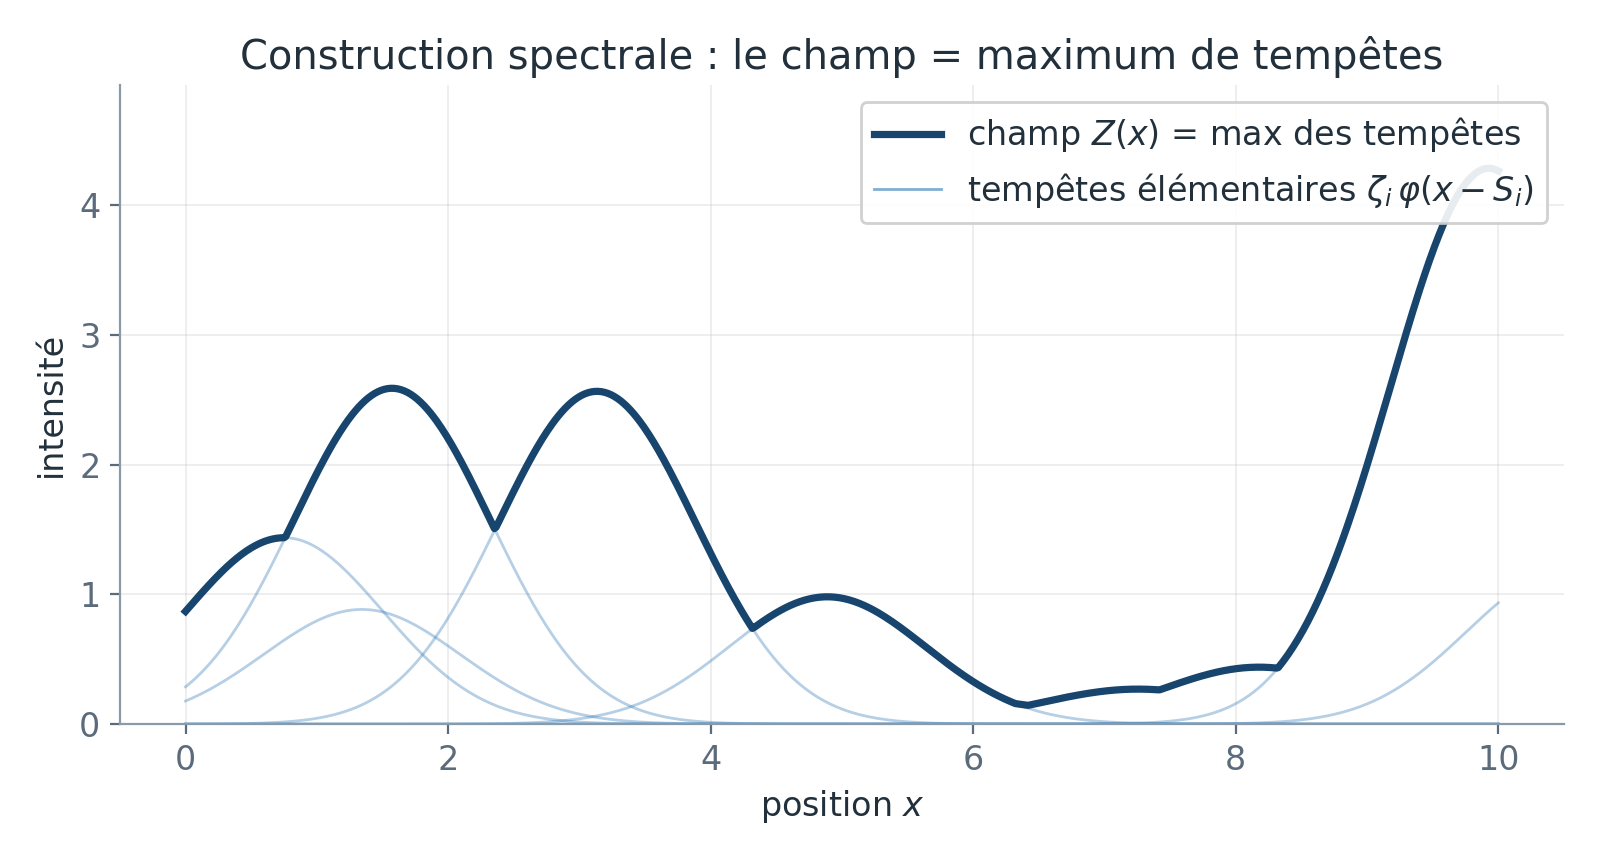
\includegraphics[width=0.82\linewidth]{fig1_construction_spectrale_1d}
  \caption{Construction spectrale en dimension~1 (modèle de Smith). Les courbes
  claires sont les tempêtes élémentaires $\zeta_i\,\varphi(x-S_i)$ ; la courbe
  foncée est le champ $Z(x)$, obtenu comme leur enveloppe supérieure (maximum
  point par point).\protect\footnotemark}
  \label{fig:spectral}
\end{figure}
\footnotetext{Les figures de cette partie sont des réalisations que nous avons
simulées nous-mêmes (algorithme spectral de Poisson).}

\subsection{Le modèle de Smith}

La représentation~\eqref{eq:spectral} admet plusieurs modèles selon la forme
choisie --- Schlather, Brown--Resnick, tube ---, dont les structures de
dépendance reposent sur des fonctions de corrélation isotropes
(figure~\ref{fig:correl}). Nous nous concentrons sur le plus simple et le plus
visuel : le \emph{modèle de Smith}.

Smith correspond à un choix de forme \emph{invariant par translation} : la
fonction spectrale générale $V_{\mathbf x}(S_i)$ se spécialise en
\begin{equation}\label{eq:smith-form}
V_{\mathbf x}(S_i)=\varphi(\mathbf x-S_i),
\end{equation}
où $\varphi$ est la \emph{densité gaussienne} de covariance $\Sigma$. Chaque
tempête est donc une même « cloche » $\varphi$, simplement déplacée à sa position
$S_i$ (d'où le nom de \emph{Moving Maxima}). Le champ s'écrit alors
\[
Z(\mathbf x)=\bigvee_i U_i\,\varphi(\mathbf x-S_i).
\]

Pourquoi ce choix plutôt qu'un autre ? Pour trois raisons. D'abord la
\emph{simplicité} : une tempête est entièrement décrite par la matrice $\Sigma$,
qui règle sa taille, sa forme et son orientation. Ensuite
l'\emph{interprétabilité} : on \emph{voit} la tempête, une bosse gaussienne
lisse (figure~\ref{fig:champ2d}). Enfin le \emph{calcul} : son coefficient
extrémal admet une forme fermée, $\Theta(h)=2\,\Phi(h/2)$ (avec $\Sigma=I$), qui
tend vers $2$ à grande distance --- c'est-à-dire vers l'indépendance, donc une
diversification spatiale totale, comme on le verra plus loin.

\begin{figure}[htbp]
  \centering
  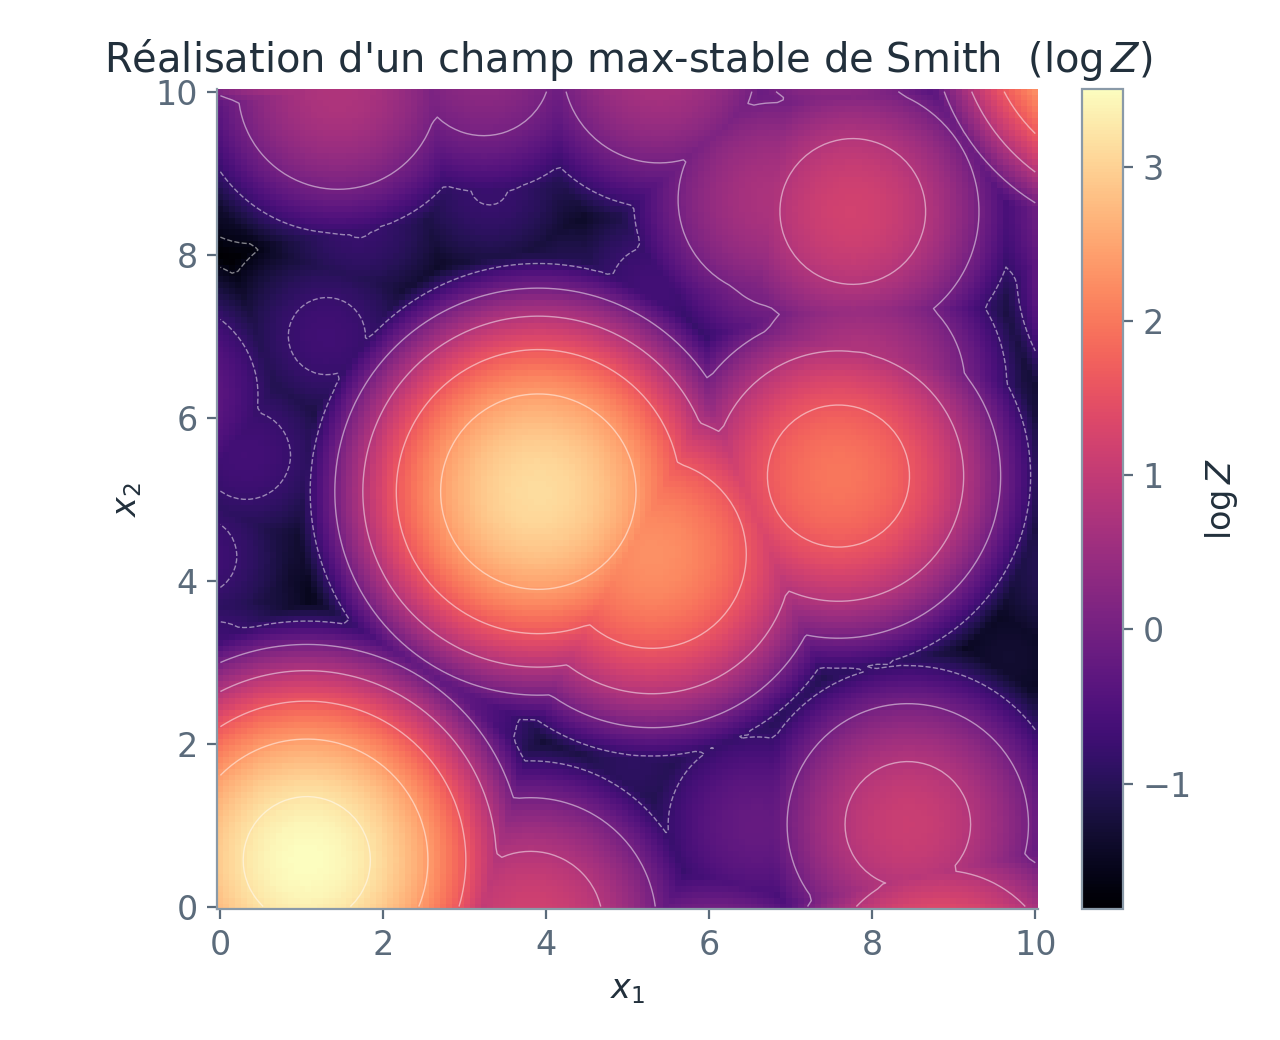
\includegraphics[width=0.60\linewidth]{fig2_champ_smith_2d}
  \caption{Réalisation d'un champ max-stable de Smith en dimension~2
  ($\Sigma=I$, échelle logarithmique). Chaque foyer clair est une tempête
  gaussienne ; le champ est leur maximum ponctuel.}
  \label{fig:champ2d}
\end{figure}

\begin{figure}[htbp]
  \centering
  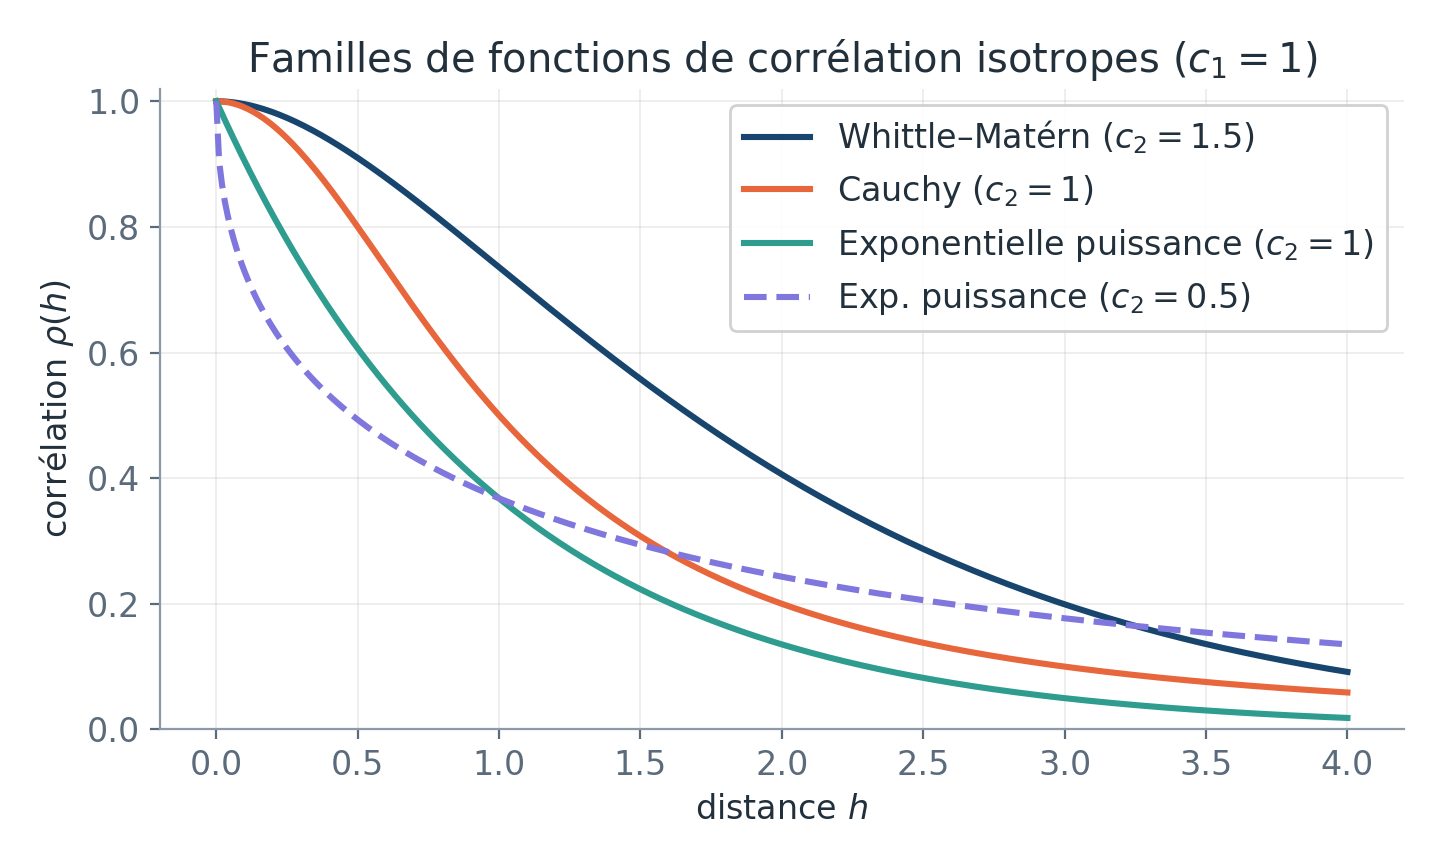
\includegraphics[width=0.72\linewidth]{fig3_fonctions_correlation}
  \caption{Familles de fonctions de corrélation isotropes ($c_1=1$), qui
  gouvernent la dépendance des modèles autres que Smith (Schlather,
  Brown--Resnick, gaussien géométrique).}
  \label{fig:correl}
\end{figure}

\subsection{Vers la dépendance spatiale}

La quantité qui résume la dépendance spatiale des extrêmes est le
\emph{coefficient extrémal} $\Theta$, défini par la loi bivariée
\begin{equation}\label{eq:theta-def}
\PP\bigl(Z(\mathbf x_1)\le u,\ Z(\mathbf x_2)\le u\bigr)
=\exp\!\left(-\frac{\Theta(\mathbf x_1,\mathbf x_2)}{u}\right),
\qquad \Theta\in[1,2].
\end{equation}
La valeur $\Theta=1$ correspond à la dépendance parfaite (les deux sites sont
extrêmes ensemble), $\Theta=2$ à l'indépendance. Pour un processus stationnaire
et isotrope, $\Theta$ ne dépend que de la distance
$h=\|\mathbf x_1-\mathbf x_2\|$ et croît de $1$ à $2$
(figure~\ref{fig:theta}). C'est cet objet, et son lien avec le mélange
(\emph{mixing}) du processus, qui gouverne la diversification spatiale étudiée
dans la partie suivante.

\begin{figure}[htbp]
  \centering
  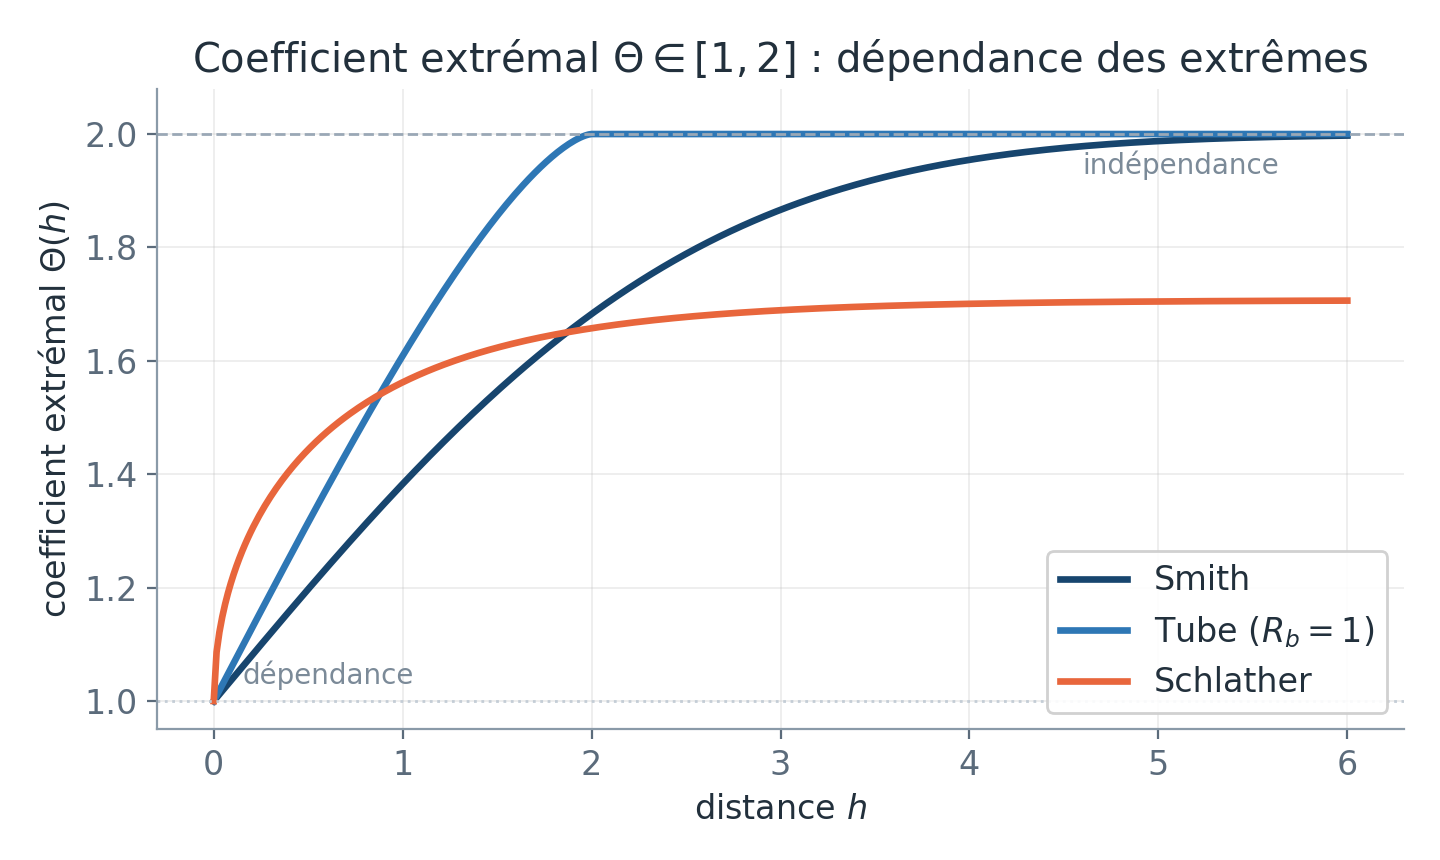
\includegraphics[width=0.72\linewidth]{fig4_coefficient_extremal}
  \caption{Coefficient extrémal $\Theta(h)$ pour trois modèles : il croît de la
  dépendance ($\Theta=1$) vers l'indépendance ($\Theta=2$) avec la distance ; le
  modèle tube atteint l'indépendance à distance finie.}
  \label{fig:theta}
\end{figure}

\end{document}